\documentclass[11pt]{amsart}

\usepackage{amssymb}
\usepackage{amsthm}
\usepackage{amsmath}

%\usepackage[margin=1in]{geometry}

\usepackage[usenames]{color}
\usepackage{tikz}

\usepackage{hyperref}

\theoremstyle{plain}
\newtheorem{proposition}{Proposition}[section]
\newtheorem{theorem}[proposition]{Theorem}
\newtheorem{lemma}[proposition]{Lemma}
\newtheorem{corollary}[proposition]{Corollary}
\theoremstyle{definition}
\newtheorem{example}[proposition]{Example}
\newtheorem{exercise}[proposition]{Exercise}
\newtheorem{definition}[proposition]{Definition}
\newtheorem{observation}[proposition]{Observation}
\theoremstyle{remark}
\newtheorem{remark}[proposition]{Remark}
\newtheorem{fact}[proposition]{Fact}
\newtheorem{conjecture}[proposition]{Conjecture}
\newtheorem{question}[proposition]{Question}
\newtheorem{problem}[proposition]{Problem}


\DeclareMathOperator{\id}{id}
\DeclareMathOperator{\stab}{stab}
\DeclareMathOperator{\diam}{diam}
\DeclareMathOperator{\cuspdepth}{CuspDepth}

\DeclareMathOperator{\dist}{d}
\DeclareMathOperator{\CAT}{\mathsf{CAT}}
\DeclareMathOperator{\Isom}{\mathsf{Isom}}
\DeclareMathOperator{\PSL}{\mathsf{PSL}}
\DeclareMathOperator{\SL}{\mathsf{SL}}


%%%%%%%%%%%%%%%%%%%%%%%%%%%%%%%%%%%%%%%%%%%%%%%%%%%%%%%%%%%%%%%%%%%%%%%%%%%%%%%%%%%%%%%%%%%%%%%%%%%%%%%%%%%%%%%%%

\newcounter{countharry}
\setcounter{countharry}{1}
\newcommand{\comharry}[1]{{\textcolor{red}{\textrm{{\bf (\arabic{countharry})\stepcounter{countharry} Harry:} #1}}}}


\newcounter{countchenxi}
\setcounter{countchenxi}{1}
\newcommand{\comchenxi}[1]{{\textcolor{blue}{\textrm{{\bf
(\arabic{countchenxi})\stepcounter{countchenxi} Chenxi:} #1}}}}


%%%%%%%%%%%%%%%%%%%%%%%%%%%%%%%%%%%%%%%%%%%%%%%%%%%%%%%%%%%%%%%%%%%%%%%%%%%%%%%%%%%%%%%%%%%%%%%%%%%%%%%%%%%%%%%%

\date{\today}

\begin{document}

\title[A 0-1 law for hyperbolic metric spaces]{
  A 0-1 law and cusp excursion for geometrically finite actions on coarsely
  hyperbolic metric spaces
}
\author{Harrison Bray}
%\address{.}
%\email{}
\date{\today}
\keywords{}
\subjclass[2020]{}

\begin{abstract} 
  Based on joint work with Giulio Tiozzo.
\end{abstract}

\maketitle

\tableofcontents

\section{Introduction}

\subsection{History}


Given a function $\psi\colon\mathbb N\to \mathbb R+$, define
\[ 
  \Theta(\psi)=\{x\in\mathbb [0,1] : |x-\frac{p}q|<\frac{\psi(q)}q
  \text{ for infinitely many reduced rationals }\frac{p}q \}
\]
Note that if $\psi\equiv 1$ then $\Theta(\psi)=[0,1]$. A century ago,
Khinchin proved the following celebrated theorem: 

\begin{theorem}[Khinchin, 1926]
  Let $\psi\colon \mathbb N\to\mathbb R^+$ be monotone decreasing.
  \comharry{is this even needed? any other hypotheses?}
  Then 
  \[
    \sum_{q\in\mathbb N} \psi(q)=\infty \; \text{ then }\; \Theta(\psi)
    \text{ has measure 1}
  \]
  and 
  \[
    \sum_{q\in\mathbb N} \psi(q)=0 \; \text{ then }\; \Theta(\psi)
    \text{ has measure zero}.
  \]
  \label{thm:khinchin}
\end{theorem}

Thus, Theorem~\ref{thm:khinchin} is a strong 0-1 law for the interval. As
an application, we have the following classical example: 

\begin{example}
  Let $\psi_\epsilon(q)=q^{-(1+\epsilon)}$. Then 
  \[
    \Theta(\psi_\epsilon)=\{
      x\in\mathbb R :
      |x-\frac{p}q|<\frac1{q^{2+\epsilon}}
      \text{ 
	for infinitely many
      }\frac{p}q\in\mathbb Q
    \}.
  \]
  Let us illustrate the limsup set $\Theta(\psi_0)$. 

  \begin{figure}[h!]
    \centering
        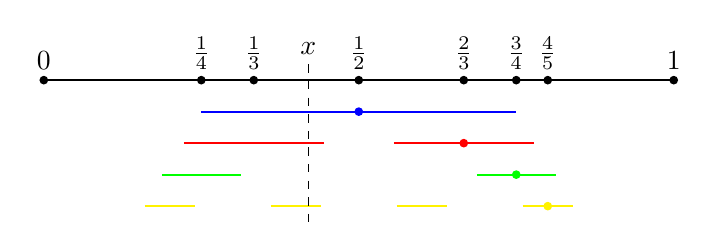
\begin{tikzpicture}[scale=8,thick]
    \draw[-] (0,0)--(1,0); 
    \def\s{.005}

    \def\e{.05}
    \draw[blue] (.25,-\e)--(.75,-\e);
    \draw[fill,blue] (.5,-\e) circle (\s) node {};


    \begin{scope}[red]
      \draw[] (.555555,-2*\e)--(.77777,-2*\e);
      \draw[] (.33333-.111111,-2*\e)--(.333333+.111111,-2*\e);
      \draw[fill] (.6666667,-2*\e) circle (\s) node {};
    \end{scope}

    \begin{scope}[green]
    \draw[] (.6875,-3*\e)--(.8125,-3*\e);
    \draw[fill] (.75,-3*\e) circle (\s) node {};

    \draw[] (.25-0.0625,-3*\e)--(.25+0.0625,-3*\e);
    \end{scope}


    \begin{scope}[yellow]
      
    \draw[] (.76,-4*\e)--(.84,-4*\e);
    \draw[fill] (.8,-4*\e) circle (\s) node {};

    \draw[] (.2-.04,-4*\e)--(.2+.04,-4*\e);
    \draw[] (.4-.04,-4*\e)--(.4+.04,-4*\e);
    \draw[] (.6-.04,-4*\e)--(.6+.04,-4*\e);

    \end{scope}

    \draw[fill] (0,0) circle (\s) node[above] {$0$};
    \draw[fill] (1,0) circle (\s) node[above] {$1$};
    \draw[fill] (.25,0) circle (\s) node[above] {$\frac14$};
    \draw[fill] (.33333,0) circle (\s) node[above] {$\frac13$};
    \draw[fill] (.5,0) circle (\s) node[above] {$\frac12$};
    \draw[fill] (.666667,0) circle (\s) node[above] {$\frac23$};
    \draw[fill] (.75,0) circle (\s) node[above] {$\frac34$};
    \draw[fill] (.8,0) circle (\s) node[above] {$\frac45$};


    \draw[dashed,thin] (.42,.5*\e) node[above] {$x$} -- (.42,-4.5*\e);
  \end{tikzpicture}

    \caption{
      An illustration of the first levels of the limsup set
      $\Theta(\psi_0)$. The intervals around $\frac12$ have radius $\frac14$,
      around $\frac23$ have radius $\frac19$, and so on.
    }
    \label{fig:khinchin}
  \end{figure}

  See that 
  \[
    \sum_{q\in\mathbb N}\psi_\epsilon(q)=\sum_{q\in\mathbb
    N}\frac1{q^{1+\epsilon}}
     \left\{
      \begin{array}[]{cc}
	=\infty & \text{ for }\epsilon=0\\
	<\infty & \text{ for }\epsilon>0
      \end{array}
    \right.
  \]
  hence
  Khinchin's theorem implies 

  \[
    \Theta(\psi_\epsilon) \text{ has measure }
    \left\{
      \begin{array}[]{l}
	\text{  one for }\epsilon=0 \\
	\text{  zero for }\epsilon>0.
      \end{array}
    \right.
  \]

  Thus in Figure~\ref{fig:khinchin}, $x$ is in infinitely many balls of radius
  $\frac1{q^2}$ about $\frac{p}q$ with probability 1. 

\end{example}

We will now discuss an analogy of Khinchin's Theorem (\ref{thm:khinchin})
for the hyperbolic plane, due originally to Sullivan \cite{sullivan84}.


\subsection{Horoball packings at infinity for hyperbolic 2-space} 

The results of Sullivan generalize but we present them for surfaces, or
really for a particular surface, to communicate the concept. A statement
in full generality appears \comharry{ref} and is the goal of these notes. 

Let $\mathbb D$ denote the disk model of hyperbolic 2-space. 
Recall a { \em  Fuchsian group} is a discrete subgroup $\Gamma$ of 
$\Isom(\mathbb D)$ acting by 
%$\PSL(2,\mathbb
%R)$, which acts on the upper half-plane model of hyperbolic 2-space
%$\mathbb H^2$ by isometries via 
M\"obius transformations. Let
$\Sigma_{g,n}$ denote a surfaces of genus $g$ with $n$ punctures. Consider a
representation 
$\Gamma<\Isom(\mathbb D) $
%$\Gamma<\PSL(2,\mathbb R) $
of $\pi_1(\Sigma_{0,1})$ which
acts cofinitely on $\mathbb D$; that is, the quotient $\mathbb
D/\Gamma$ has finite area. In particular, let $\Gamma$ 
be a representation for which 
the ideal quadrilateral with vertices
$1,-i,1,i\in\partial \mathbb D=S^1$ is a fundamental domain for the
$\Gamma$-action. 


We now introduce a concept of horoball packing at infinity. 
We will say a {\em horoball centered at $p\in S^1$} is a horoball in
$\mathbb D$ (which is a Euclidean ball in this model) tangent to $S^1$ at
$p$. 
Let $\mathcal P=\Gamma.\{\pm1,\pm i\}$. These {\em parabolic points} will be
in analogy with radional points.
For $p\in \{\pm 1,\pm i\},$ choose a collection of (sufficiently small)
horoballs $H_p$ centered at $p$. Then for $gp\in\mathcal P$, let
$H_{gp}=gH_p$. Thus we have a family $\{H_p\}_{p\in\mathcal P}$ of
horoballs, with each $H_p$ centered at $p$. Let $r_p$ denote the
Euclidean radius of $H_p$ in the disk model $\mathcal D$.
Now, to allow for rescaling, we denote by $H_p(r)$ the horoball centered at
$p$ of Euclidean radius $r$. Thus, $r_p$ is chosen so that
$H_p=H_p(r_p)$. Finally, we define the {\em horoball shadow $\mathcal
H_p(r)$ centered at $p$ with radius $r$} to be the set of a endpoints
$\xi$ of
geodesic rays $[0,\xi)$ such that $[0,\xi)$ intersects the horoball
$H_p(r)$ in $\mathbb D$. See that $\mathcal H_p(r)$ is an
interval in $S^1$ centered at $p$ with radius approximately $r$. 

\subsection{0-1 law and cusp excursion in hyperbolic 2-space}
Now, for $\phi\colon\mathbb R^+\to\mathbb R^+$ \comharry{increasing and?}
we define the limsup set

\[
  \Theta(\phi)=\{x\in S^1 : x\in\mathcal H_p(r_p\phi(r_p)) \text{ for
  infinitely many }p\in\mathcal P\}. 
\]

When $\phi\equiv 1$, $\Theta(1)$ is the shadows of all the horoballs from
the original packing, without any rescaling. These horoballs all project to
the same horoball neighborhood of the cusp in the punctured torus quotient. 
It is a fact due to ergodicity
of the geodesic flow of $\Sigma_{0,1}$ 
that in this case, Lebesgue-almost every geodesic visits each
horoball infinitely often. Hence, $\Theta(1)$ has Lebesgue measure 1. We 
should think of $r_p$ as analogous to the standard radius $\frac1q$ of
$\frac{p}q$ for the corresponding limsup set for the real line. 

The following 0-1 for hyperbolic 2-space is due to Sullivan:

\begin{theorem}[Khinchin]
  For sufficiently small $\lambda\in (0,1)$, 
  Then 
  \[
    \sum_{n\in\mathbb N} \phi(q)=\infty \; \text{ then }\; \Theta(\phi)
    \text{ has Lebesgue measure 1}
  \]
  and 
  \[
    \sum_{n\in\mathbb N} \phi(q)=0 \; \text{ then }\; \Theta(\phi)
    \text{ has Lebesgue measure zero}.
  \]
  \label{thm:khinchin_type}
\end{theorem}

This theorem provides an application to cusp excursion called the {\em logarithm
law}. First, define the {\em non-cuspidal} part of $\mathbb D$ to be 
\[
  NC=\mathbb D \smallsetminus \cup_{p\in\mathcal P} H_p.
\]

Then for a point $x\in \mathbb D$, define the $\cuspdepth(x)$
to be 0 if $x\in NC$, and 
\[
  \cuspdepth(x)=d(x,\partial H_p) \; \text{ where } x\in H_p.
\]
Given a point $\xi\in S^1$, denote by $\xi_t$ the point on the geodesic ray
$[0,\xi)$ which is distance $t$ from $0$. 

\begin{theorem}
  For Lebesgue almost every $\xi\in S^1$, 
  \[
    \limsup_{t\to+\infty} \frac{\cuspdepth(\xi_t)}{\log t}=1.
  \]
  \label{thm:loglaw}
\end{theorem}


\subsection{Overview of the notes}

With Tiozzo, we generalize Theorems~\ref{thm:khinchin_type} and
\ref{thm:loglaw} to the setting of certain geometrically finite actions on
coarsely hyperbolic metric spaces.  In these notes, I present the proof
strategy for these results at that level of generality. I introduce the
setting with fundamental intuition and examples. Along the way I review
some of the foundational Patterson--Sullivan theory needed for these
results. 

\section{Hyperbolic metric spaces}

For a more complete treatment of hyperbolic metric spaces,
\comharry{add refs} 

First for any set $U$ and functions $f,g\colon U\to \mathbb R$, we write 
\begin{itemize}
  \item $f\approx g$ if there exists a constant $C$ such that $f-C\leq g\leq
    f+C$ on $U$, and 
  \item $f\asymp g$ if there exists a constant $K$ such that $\frac1Kf\leq
    g\leq Kf$. 
\end{itemize}

Recall that a metric space $(X,d)$ is {\em (Gromov) hyperbolic} or {\em
$\delta$-hyperbolic} if there exists a $\delta>0$ such that all geodesic
triangles in $X$ are $\delta$-thin: more specifically, for any geodesic
triangle $\Delta$ with vertices $x,y,z\in X$,
any edge $[x,y]$ of $\Delta$ is contained in the
$\delta$-neighborhood of the two other edges $[y,z]\cup [x,z]$ 
of $\Delta$. For example,
trees are 0-hyperbolic, and $\mathbb H^2$ is $\log 2$-hyperbolic. One
should think of a hyperbolic metric space as coarsely a tree. 

As an alternate definition, $(X,d)$ is Gromov-hyperbolic if and only if
for every geodesic triangle $\Delta$ with vertices $x,y,z\in
X$, there exist three points
$a\in[x,y],b\in[y,z]$, and $c\in[x,z]$ such that $\diam(\{a,b,c\})\leq
\delta$. A geodesic triangle with vertices $a,b,c$ is said to be an
{\em inner triangle} of $\Delta$. Note that for a tree, we have $a=b=c$. 

Given a triple $x,y,z\in X$, {\em the Gromov product} is 
\[
  \langle x,y\rangle_z=\frac12(d(x,z)+d(y,z)-d(x,z)).
\]

Notice that for a tree, $\langle x,y\rangle_z=d(z,[x,y])$. More
generally, 
the Gromov product measures the defect from colinearity of the triple
$x,y,z$, up to additive error:  


\begin{fact}
  For a $\delta$-hyperbolic metric space $(X,d)$, 
  \[
    \langle x,y\rangle_z\approx d(z,[x,y])
  \]
  with constants depending only on $\delta$. 
\end{fact}


Fixing a perspective point $o\in X$, the {\em visual boundary} of
$X$ is denoted by $\partial X$, and is the set of geodesic rays based at
$o$ up to bounded equivalence. Define the {\em shadow} $\mathcal
O_r(x,y)$ of $y\in X$ of
radius $r$ by 
\[
  \mathcal O_r(x,y)=\{\xi\in\partial X\mid [x,\xi)\cap B_r(y)\neq \varnothing
    \text{ for some geodesic representation }[x,\xi)\text{ of }\xi
\}.
\]

The notation $\mathcal O$ stands for ombre, which is French for shadow. 
The visual boundary is a compactification of
$X$ when endowed with the shadow topology. Let $\bar{X}=X\cup\partial X$. 

\subsection{Busemann functions and horoballs}

The notion of horoball in a hyperbolic metric space is defined using
Busemann functions. This generalizes the setting of hyperbolic space and
shares many essential properties.

For $x,y,z\in X$, define the {\em Busemann function} centered at $z$ by 
\[
  \beta_z(x,y)=d(x,z)-d(y,z).
\]
This expression measures the signed distance between spheres centered at
$z$ passing through $x$ and $y$. 
Let $\xi\in \partial X$. Then 
\[
  \beta_\xi(x,y)=\liminf_{z\to\xi} \beta_z(x,y). 
\]

In hyperbolic space, $\beta_\xi$ is in fact a limit. In general it is not.
For example, one could take the infinite graph given by a ladder with
infinitely many rungs and the standard path metric. This space is 
hyperbolic (it is quasi-isometric to a tree), but the Busemann function is
not a limit. It is nonetheless well-defined up to choice of path:

\begin{fact}
  In a $\delta$-hyperbolic metric space, for any two sequences
  $z_,w_n\to\xi\in\partial X$, 
  \[
    \beta_{z_n}(x,y)\approx\beta_{w_n}(x,y)
  \]
  with constants depending only on $\delta$. 
\end{fact}

Some straightforward but useful 
properties of Busemann functions include:

For all $x,y,w\in X$, $z\in \bar{X}$, 
\begin{enumerate}
  \item ($\Gamma$-invariant) $\beta_{\gamma z}(x,y)=\beta_z(x,y)$ for all
  \item (asymmetric) $\beta_z (x,y) \approx -\beta_z(y,x)$. 
  \item (1-Lipshitz) $|\beta_z(x,y)|\leq d(x,y)$. 
  \item (cocycle property) $\beta_z(x,y)\approx
    \beta_z(x,w)+\beta_z(w,y)$.
\end{enumerate}

Notice that the $1$-Lipshitz property implies finiteness of $\beta_\xi$ for
$\xi\in\partial X$. 


\begin{definition}
  Fixing $o\in X$, the {\em horoball of radius $r$ centered at $\xi$} is 
  \[
    H_\xi(r)=\{x\in X\mid \beta_\xi(x,o)\leq \log r\}. 
  \]
  A {\em horosphere of radius $r$ centered at $\xi$} 
  $\{x\in X\mid \beta_\xi(x,o)=\log r\}. $
  \label{def:horoball}
\end{definition}


We think of horospheres
as a limit of metric spheres $S_n$
which contain a fixed point $x$, with each sphere $S_n$
centered at 
$z_n$ which are 
going to $\partial X$ with $n$.
It is straightforward to verify that in 
$\mathbb R^2$, horospheres are lines, and horoballs are 
halfspaces. In $\mathbb D$, horospheres are Euclidean circles tangent to
the boundary $S^1$, and horoballs are the disks contained in these circles.
In the upper-half space model $\mathbb H^2$ 
of hyperbolic 2-space, horospheres centered
at the vertical point at infinity are horizontal lines, and all other
horospheres are Euclidean circles tangent to the real line. In particular,
a straightforward exercise is to confirm in $\mathbb H^2$ that for $o=i$ and  $\xi=0$, we
have $H_\xi(2r)$ is a Euclidean ball of radius $r$ about $ir$. 
This motivates the choice of
$\log r$ in the definition of the horoball.


\begin{definition}
  The {\em shadow of a horoball of radius }$r$ centered at $\xi$ is 
  \[
    \mathcal H_\xi(r):=\{\eta\in\partial X\mid [o,\eta)\cap H_\xi(r)\neq \varnothing
    \text{ for some geodesic representative of }\eta\}.
  \]
  \label{def:horoball_shadows}
\end{definition}

\subsection{Geometrical finiteness}


Fix a group $\Gamma$ of isometries of a hyperbolic metric space $(X,d)$
acting properly discontinuously. 
Assume $(X,d)$ is proper. 
The {\em limit set} of $\Gamma$ is the set of accumulation points of
a $\Gamma$-orbit:
\[
  \overline{\Gamma.o}/\Gamma.o 
\]
for any fixed $o\in X$. 
By proper discontinuity, $\Lambda_\Gamma\subset\partial X$.
Since $X$ is hyperbolic, $\Lambda_\Gamma$ does not
depend on the basepoint \comharry{Coornaert Th\'eor\`eme 5.1}. 
The group $\Gamma$ is {\em non-elementary} if $|\Lambda_\Gamma|\geq 3$.
Equivalently, $\Gamma$ does not fix any point. \comharry{add refs}
It follows that $\Lambda_\Gamma$ is uncountable. 
When $\Gamma$ is non-elementary, $\Lambda_\Gamma$ is the
smallest closed $\Gamma$-invariant subset of $\partial X$. 
Let $C_\Gamma$ denote the {\em convex hull} of $\Lambda_\Gamma$; this is
the intersection with $X$ of the smallest convex set in $\bar{X}$
containing $\Lambda_\Gamma$. 

Isometries of $X$ are classified by their translation distance. The
{\em translation distance} of $\gamma\in\Isom(X)$ is
$\tau(\gamma)=\inf_{o\in X}d(o,\gamma o)$. Then $\gamma$ is {\em elliptic}
if $\tau(\gamma)=0$ is realized in $X$, {\em parabolic} if $\tau(\gamma)=0$
is not realized, and {\em hyperbolic} or {\em loxodromic}
if $\tau(\gamma)>0$, which implies in this setting that it is realized in
$X$. If $\gamma$ is parabolic then it is infinite order with a single fixed
point in $\partial X$, and if $\gamma$ is loxodromic then $\gamma$ is
infinite order with each two fixed points in $\partial X$, one attracting
and one repelling. \comharry{Bowditch Lemma 2.1}
A subgroup $\Pi$ of $\Isom(X)$ is a {\em parabolic group} if  $\Pi$ has
infinite order, fixes a single point in $\partial X$, and contains no
loxodromic elements.


A point $x\in\Lambda_\Gamma$ is {\em conical} if for any geodesic ray
$\xi$ in the class of $x$, there exists a constant $D$ and a sequence
$x_n\in\Gamma.o$ converging to $x$ such that $\{x_n\}_{n\in\mathbb
N}$ is contained in a $D$ neighborhood of $\xi$. Equivalently, $x$ is
conical in the sense of a convergence group action; in particular, there
exists a sequence $\gamma_n\in\Gamma$ and $a\neq b\in\Lambda_\Gamma$ such
that $\gamma_n x\to a$ and $\gamma_n y\to b$ for all
$y\in\Lambda_\Gamma\smallsetminus\{x\}$.   

\begin{exercise}
  \begin{enumerate}
    \item 
      If $\gamma\in\Isom(\mathbb H^2)$ is
      loxodromic, then the attracting and repelling fixed points of $\gamma$ are
      conical limit points for any subgroup of isometries containing $\gamma$. 
    \item 
      Verify that every fixed point of a parabolic
      isometry is in $\Lambda_\Gamma$. 
    \item Assume $g$ is loxodromic, $h$ is parabolic and
      $g,h\in\Gamma$. If 
      $\Gamma$ is properly discontinuous then 
      $g$ and $h$ cannot fix a common point in $\Lambda_\Gamma$. 
  \end{enumerate}

\end{exercise}
Then a point $x\in\Lambda_\Gamma$ is {\em parabolic} if its stabilizer
$\stab_\Gamma(x)$ is a parabolic subgroup, and is moreover {\em bounded
parabolic} if $\Gamma$ acts on $\Lambda_\Gamma\smallsetminus\{x\}$
cocompactly. 

\begin{example}
A first example for a parabolic subgroup is $\langle z\mapsto z+1\rangle$
acting on the upper-half plane, which fixes $\infty$. Every
parabolic isometry in this model is conjugate to a horizontal translation,
which is upper triangular as a matrix. 
Every loxodromic isometry is conjugate to a scaling $z\mapsto \lambda
z$ for some $\lambda>0$, which is diagonal as a matrix. 

In $\mathbb H^3$, \comharry{discuss a $\mathbb Z^2$ subgroup}. Remark that
parabolic subgroups in $\mathbb H^n$ are virtually abelian with rank
$\leq n-1$. 
\end{example}


Then $\Gamma$ is {\em geometrically finite} if every point of
$\Lambda_\Gamma$ is either conical or bounded parabolic, and $\Gamma$ is
more specifically {\em convex cocompact} if every point in $\Lambda_\Gamma$
is conical. 
Classically, for Kleinian groups $\Gamma<\mathbb H^3$, Beardon--Maskit
proved that $\Gamma$ is geometrically finite if and only if $\Gamma$ admits
a polygonal fundamental domain with finitely many sides. For higher
dimensions this is false, but the framework of geometrical finiteness is
fairly robust.  

We discuss some examples below, but first here are some crucial facts that
will be enlightened via examples. 

\begin{fact}[Tukia, Yaman, Bowditch]
  {\color{red}
    finitely many cusps

    horoball packing 

    cocompact action on noncuspidal part
  }
\end{fact}


Here are some examples.
First, every finite covolume action on $\mathbb H^n$ is geometrically
finite. 
A good example to have in mind is the punctured torus, with genus 1
and 1 puncture, denoted $\Sigma_{1,1}$. This surface 
admits a hyperbolic metric of
finite area by choosing opposite edge identifications for an ideal
quadtrilateral, for instance as
pictured in
\comharry{figure}. The corresponding representation of $\pi_1(S)$ is
computable; the generators are loxodromic with axes intersecting the
identifying edges orthogonally.
The one can verify that the commutators of this representation are parabolic,
and in particular there is one commutator which is equal to a horizontal
translation. 
In $\mathbb H^2$, when $\Gamma$ has parabolics, 
by definition this introduces a cuspidal region to the quotient, which
lifts to a $\Gamma$-invariant collection of horoballs in $\mathbb H^2$,
each preserved by a parabolic subgroup. 
Since the property of being a parabolic fixed point is
$\Gamma$-invariant,
by computating the representation we confirm that 
the rationals are parabolic, hence
$\Lambda_\Gamma=\partial H^2=S^1$. Now it is straightfoward to verify that
the parabolic points are bounded parabolic. The fact that all other points
in $S^1$ are conical follows from \comharry{the fact}

\begin{exercise}
Verify that 
when $\Gamma$ is cocompact, $\Lambda_\Gamma=\partial X$ and hence
$C_\Gamma=X$. By the translation distance definition, $\Gamma$ has no
parabolic isometries.  
\end{exercise}

It follows from the previous exercise 
that cocompact actions are the first examples of convex
cocompact actions, and that moreover 
$\Gamma$ is convex cocompact if and only if the Cayley graph of $\Gamma$
is quasi-isometrically embedded in $X$ via the orbit map
$\gamma\mapsto\gamma.o$. 
We can think of geometrical
finiteness as a natural extension of convex cocompactness 
where orbits do not quasi-isometrically
embed  but the action retains some
finiteness properties. 

\begin{exercise}
  Orbits of the parabolic subgroup $G=\langle z\mapsto z+1\rangle$  acting on
  $\mathbb H^2$ grow logarithmically in $n$, and hence the orbit map does
  not quasi-isometrically embed. 
\end{exercise}

\subsection{Growth conditions}

To state the results, we will need to assume some growth conditions on the
parabolic subgroups. 
For a parabolic subgroup $\Pi<\Gamma$, define the growth function by 
\[
  B_\Pi(t)=\#\{g\in \Pi \mid d(o,go)\leq t\}.
\]
Then $\Pi$ has 
{\em mixed exponential growth} if there exist $a_\Pi,\delta_\Pi$ such that 
\[
  B_\Pi(t)\asymp e^{\delta_\Pi t}(t+1)^{a_\Pi}. 
\]

\begin{exercise}
  If $\Pi$ is a parabolic subgroup acting on $\mathbb H^2$ then
  $\delta_\Pi=\frac12$ and $a_\Pi=0$. More generally, if $\Pi$ acts on
  $\mathbb H^n$ then $\delta_\Pi=\frac{r}{n}$ where $r$ is the abelian rank
  of $\Pi$.
\end{exercise}



\begin{example}
[Groves--Manning cusp space]
Here is a another example of a geometrically finite group action 
which allows for many possible growth functions. 

\end{example}


Though our theorems are more general, we will present the notes under these
growth assumptions for ease of readability, and refer the reader to
\comharry{b-t} for details in greater generality. 





\comharry{resume on page 8 with the facts of Tukia, Yaman, Bowditch}





\bibliographystyle{plain}
\bibliography{refs}


\end{document}



